\section{Decomposable Graphs}
\label{sec:treewidth}

In this chapter, we introduce the notion of treewidth and decomposable graphs. Section \ref{sec:treewidth:treewidth} defines a tree decomposition and recapitulates some well-known properties and results. After this, we define the class of decomposable graphs in Section \ref{sec:treewidth:decompgraphs}. 

\subsection{Treewidth}
\label{sec:treewidth:treewidth}

Informally speaking, the treewidth of a graph is a measure of how ``similar" the graph is to a tree. We refer to \cite{Bod96} for a comprehensive introduction to treewidth. Since the introduction of the concept of treewidth, bounding the treewidth has been widely used to obtain polynomial time algorithms for problems that are otherwise \NP-complete. In order to formally define the treewidth of a graph, we need to introduce the structure of a tree decomposition.

\begin{definition}[Tree Decomposition]
	\label{def:treedecomp}
	Let $G = (V,E)$ be a graph. A \textit{tree decomposition} of $G$ is a pair $D = (S, T)$, where $S = \{X_i : i \in I\}$ is a family of subsets of $V$ and $T = (I,F)$ is a tree with the following properties:
	\begin{enumerate}
		\item \textit{Node coverage}. $\bigcup_{i \in I} X_i = V$.
		\item \textit{Edge coverage}. For every edge $e = (v,w) \in E$, there is a subset $X_i, i \in I$, with $v	\in X_i$ and $w \in X_i$.
		\item \textit{Coherence}. For all $i, j, k \in I$ it holds that if $j$ lies on the path from $i$ to $k$ in $T$, then $X_i\cap X_k \subseteq X_j$.
	\end{enumerate}
	We call the $X_i$ the \textit{bags} of the tree decomposition.
\end{definition}

\begin{definition}[Treewidth]
	The \textit{width} of a tree decomposition $D = (S, T)$, $S = \{X_i : i \in I\}$ for a graph $G$ is defined as
	$$\mathrm{width} (D) \defeq \max_{i \in I} |X_i| - 1.$$
	The \textit{treewidth} of $G$ is denoted by 
	$$\mathrm{tw}(G) \defeq \min_{D\text{ tree decomp.}} \mathrm{width}(D)$$
	and is the minimum width of all tree decompositions for $G$.
\end{definition}

\begin{example}
	\label{ex:treedecomp}
	Figure \ref{fig:treedecomp} gives an example of a graph $G$ and two possible corresponding tree decompositions. $G$ has eight vertices and both decompositions $D_1$ and $D_2$ are trees with six bags. Each bag lists at most three vertices, so the width of these decompositions is two: $\mathrm{width} (D_1) = \mathrm{width} (D_2) = 2$.
	
	\begin{figure}[H]
		\begin{minipage}[t]{.33\linewidth}
			\centering
			\begin{tikzpicture}[scale=0.8]
			\node[circle] (a) at (0,3) {A};
			\node[circle] (b) at (1.5,5) {B};
			\node[circle] (c) at (1.5,3) {C};
			\node[circle] (d) at (3,5) {D};
			\node[circle] (e) at (1.5,1) {E};
			\node[circle] (f) at (3,3) {F};
			\node[circle] (g) at (3,1) {G};
			\node[circle] (h) at (4.5,5) {H};
			
			\foreach \from/\to in {a/b,a/c,b/c,b/d,c/d,c/e,d/f,d/h,e/g,f/g}
			\draw[] (\from) -- (\to);
			\end{tikzpicture}
			\subcaption{Input graph $G$.}\label{fig:treedecomp:graph}
		\end{minipage}%
		\begin{minipage}[t]{.33\linewidth}
			\centering
			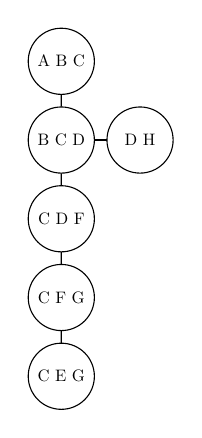
\begin{tikzpicture}[every node/.style={inner sep=1pt, minimum size=1.4cm, scale=0.6}]
			\node[circle, draw] (abc) at (0,4) {A B C};
			\node[circle, draw] (bcd) at (0,3) {B C D};
			\node[circle, draw] (dh) at (1,3) {D H};
			\node[circle, draw] (cdf) at (0,2) {C D F};
			\node[circle, draw] (cfg) at (0,1) {C F G};
			\node[circle, draw] (ceg) at (0,0) {C E G};
			
			\foreach \from/\to in {abc/bcd,bcd/dh,bcd/cdf,cdf/cfg,cfg/ceg}
			\draw[] (\from) -- (\to);
			\end{tikzpicture}
			\subcaption{Tree-decomposition $D_1$.}\label{fig:treedecomp:tree1}
		\end{minipage}
		\begin{minipage}[t]{.33\linewidth}
			\centering
			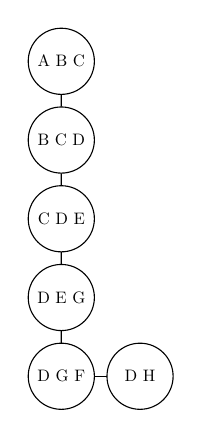
\begin{tikzpicture}[every node/.style={inner sep=1pt, minimum size=1.4cm, scale=0.6}]
			\node[circle, draw] (abc) at (0,4) {A B C};
			\node[circle, draw] (bcd) at (0,3) {B C D};
			\node[circle, draw] (dh) at (1,0) {D H};
			\node[circle, draw] (cde) at (0,2) {C D E};
			\node[circle, draw] (deg) at (0,1) {D E G};
			\node[circle, draw] (dgf) at (0,0) {D G F};
			
			\foreach \from/\to in {abc/bcd,bcd/cde,cde/deg,deg/dgf,dgf/dh}
			\draw[] (\from) -- (\to);
			\end{tikzpicture}
			\subcaption{Tree-decomposition $D_2$.}\label{fig:treedecomp:tree2}
		\end{minipage}
		\caption{Input graph $G$ with two possible valid tree decompositions $D_1$ and $D_2$, both with a treewidth of $2$.}
		\label{fig:treedecomp}
	\end{figure}
	
	 A few observations can be made that can aid in the understanding of the concept of tree decompositions.
	\begin{itemize}
		\item The tree decomposition must obviously satisfy the three properties given in Definition \ref{def:treedecomp}: node coverage, edge coverage, and coherence. All vertices are present, all edges can be associated with one or more bags, and the bags containing a certain vertex induce a subtree.
		\item The trivial tree decomposition consists of a single bag containing all the vertices. This satisfies all the constraints but is not useful in practice.
		\item Any non-leaf bag splits the graph into multiple disconnected components, making it a separator for the graph.
		\item Each clique is fully contained in a bag.
		\item Some bags can be connected to the tree at multiple locations, possibly reducing the degree of a bag.
	\end{itemize}
\end{example}

While determining the exact treewidth of a graph is  \NP-complete, there are efficient algorithms that can determine whether the treewidth is at most $k$.

\begin{theorem}
	\label{thm:treewidthlineartime}
	Let $k\in N$ be a fixed constant. There exists a linear time algorithm, which decides for a graph $G$, whether $\mathrm{tw}(G) \leq k$ and if so, outputs a tree decomposition $D = (S, T)$ of $G$ with $\mathrm{width}(D) = \mathrm{tw}(G)$ and $|V(T)| \in \OO(n)$.
\end{theorem}

For the proof of Theorem \ref{thm:treewidthlineartime}, we refer to \cite{Bod96}.

\begin{observation}
	\label{obs:treedecomplineartime}
	As a consequence of Theorem \ref{thm:treewidthlineartime}, given a class of graphs $\mathcal{G}$ and constant $k \in N$ such that $\mathrm{tw}(G) \leq k$ for all $G \in \mathcal{G}$, we can compute a tree decomposition of minimum width and size $\mathcal{O}(n)$ in linear time.
\end{observation}

Up to this point, we have no information about the structure of a tree decomposition. The next definition introduces a special type of tree decomposition which is the analog of a rooted binary tree. It limits the structure to a small set of possible transitions between bags. This allows us to formulate procedures using these structural benefits.

\begin{definition}[Nice Tree Decomposition]
	\label{def:nicetreedecomp}
	Let $G = (V, E)$ be a simple undirected graph and $D = (S, T)$ a tree decomposition of $G$. $D$ is called \textit{nice} if the tree $T = (I, F)$ is rooted, binary and the following holds for every node $i \in I$:
	\begin{itemize}
		\item[(i)] If $i$ is a leaf, then $|X_i|=1$ and we call $i$ \textit{leaf bag}.
		\item[(ii)] If $i$ has one child $j$, then either
		\begin{itemize}
        	\item $X_i = X_j \cup \{v\}$ for some $v \notin X_j$ (in this case we call $i$ \textit{introduce bag}) or
        	\item $X_i = X_j \setminus \{v\}$ for some $v \in X_j$ (in this case we call $i$ \textit{forget bag}).
    	\end{itemize}
		\item[(iii)] If $i$ has two children $j_1$, $j_2$, then $X_i = X_{j_1} = X_{j_2}$ and we call $i$ a \textit{join bag}.
	\end{itemize}
\end{definition}

The nice tree decomposition remains a valid tree decomposition itself, but only allows for three different transitions between bags. Figure \ref{fig:nicetreedecompbags} illustrates the bags of a nice tree decomposition.

\begin{figure}[H]
	\begin{minipage}[t]{.49\linewidth}
		\centering
		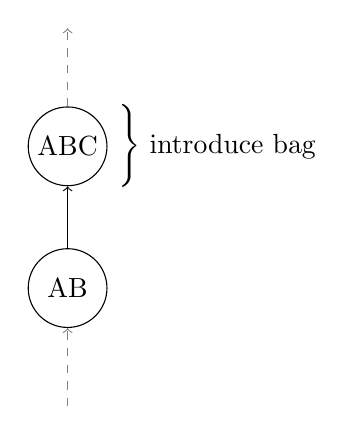
\begin{tikzpicture}
		[every node/.style={inner sep=1pt, minimum size=1cm}]
		\coordinate (leave) at (0,4.8);
		\node[circle, draw] (b) at (0,3.3) {ABC};
		\node[circle, draw] (a) at (0,1.5) {AB};
		\coordinate (enter) at (0,0);
		
		\node[right of=b, anchor=west, xshift=-0.4cm] (bracket) {$\Bigg\}$ introduce bag};
		
		\path[->] (enter) edge[dashed, gray] (a);
		\path[->] (a) edge (b);
		\path[->] (b) edge[dashed, gray] (leave);
		\end{tikzpicture}
		\subcaption{Introducing a new node.}
	\end{minipage}
	\hfill
	\begin{minipage}[t]{.49\linewidth}
		\centering
		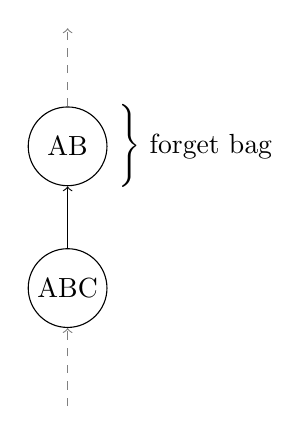
\begin{tikzpicture}
		[every node/.style={inner sep=1pt, minimum size=1cm}]
		\coordinate (leave) at (0,4.8);
		\node[circle, draw] (b) at (0,3.3) {AB};
		\node[circle, draw] (a) at (0,1.5) {ABC};
		\coordinate (enter) at (0,0);
		
		\node[right of=b, anchor=west, xshift=-0.4cm] (bracket) {$\Bigg\}$ forget bag};
		
		\path[->] (enter) edge[dashed, gray] (a);
		\path[->] (a) edge (b);
		\path[->] (b) edge[dashed, gray] (leave);
		\end{tikzpicture}
		\subcaption{Forgetting a node.}
	\end{minipage}
	\begin{minipage}[t]{\linewidth}
		\vspace{1.5cm}
	\end{minipage}
	\begin{minipage}[t]{.49\linewidth}
		\centering
		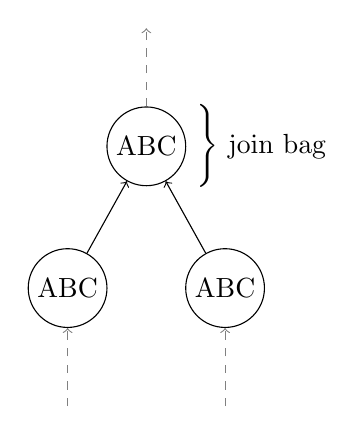
\begin{tikzpicture}
		[every node/.style={inner sep=1pt, minimum size=1cm}]
		\coordinate (leave) at (0,4.8);
		\node[circle, draw] (b) at (0,3.3) {ABC};
		\node[circle, draw] (a1) at (-1,1.5) {ABC};
		\node[circle, draw] (a2) at (1,1.5) {ABC};
		\coordinate (enter1) at (-1,0);
		\coordinate (enter2) at (1,0);
		
		\node[right of=b, anchor=west, xshift=-0.4cm] (bracket) {$\Bigg\}$ join bag};
		
		\path[->] (enter1) edge[dashed, gray] (a1);
		\path[->] (enter2) edge[dashed, gray] (a2);
		\path[->] (a1) edge (b);
		\path[->] (a2) edge (b);
		\path[->] (b) edge[dashed, gray] (leave);
		\end{tikzpicture}
		\subcaption{Joining two bags.}
	\end{minipage}
	\hfill
	\begin{minipage}[t]{.49\linewidth}
		\centering
		\begin{tikzpicture}
		[every node/.style={inner sep=1pt, minimum size=1cm}]
		\coordinate (leave) at (0,3);
		\node[circle, draw] (a) at (0,1.5) {A};
		\node[circle] (space) at (0,0) {};
		
		\node[right of=a, anchor=west, xshift=-0.4cm] (bracket) {$\Bigg\}$ leaf bag};
		
		\path[->] (a) edge[dashed, gray] (leave);
		\end{tikzpicture}
		\subcaption{Leaf of the tree decomposition.}
	\end{minipage}%
	\caption{Bags in a nice tree decomposition.}
	\label{fig:nicetreedecompbags}
\end{figure}

It is not difficult to transform a given tree decomposition into a nice tree decomposition. More precisely, the following result holds (see \cite{Kloks94}).

\begin{lemma}
	Given a tree-decomposition $D = (S, T)$ of a graph $G$, we can compute a nice tree-decomposition
	$D_0 = (S_0, T_0)$ of $G$ with
	$$\mathrm{width}(D_0) \leq \mathrm{width}(D)$$
	and
	$$|V(T_0)| \leq |V(T)| \cdot \mathrm{width}(D)$$
	in linear time.
\end{lemma}

\subsection{Decomposable Graphs}
\label{sec:treewidth:decompgraphs}

In this section, we turn to another class of graphs, the decomposable graphs. We begin by defining series-parallel graphs, which turn out to be a form of decomposable graphs. The definition of both graph classes can, for example, be found in \cite{BLW87}.

\begin{definition}[Series-Parallel Graph]
	\label{def:spg}
	The class of directed \textit{series-parallel graphs} is defined recursively as follows: A graph consisting of a single edge $(s, t)$ is \textit{series-parallel} with \textit{terminals} $s$ and $t$, called \textit{source} and \textit{sink}, respectively. If two graphs $G_1$ and $G_2$ with sources $s_1$ and $s_2$ and sinks $t_1$ and $t_2$ are series-parallel, so is their \textit{series} or \textit{parallel composition}, which are defined as follows:
	\begin{itemize}
		\item[(i)] The \textit{series composition} is obtained by taking the disjoint union of $G_1$ and $G_2$ and identifying $t_1$ and $s_2$. The new source is $s_1$ and the new sink is $t_2$.
		\item[(ii)] The \textit{parallel composition} is obtained by taking the disjoint union of $G_1$ and $G_2$ and identifying $s_1$ and $s_2$ and also $t_1$ and $t_2$. The new source is $s_1$ respectively $s_2$ and the new sink is $t_1$ respectively $t_2$.
    \end{itemize}
\end{definition}

\begin{figure}[H]
	\begin{minipage}[t]{.49\linewidth}
		\centering
		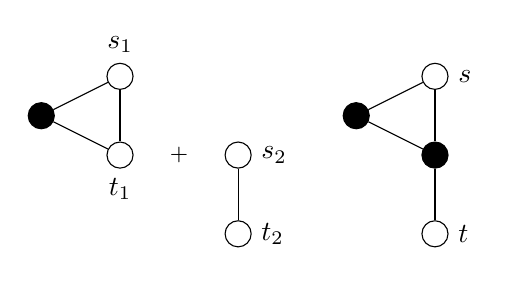
\begin{tikzpicture}
			\node[circle, draw, label=above:$s_1$] (s1) at (1,1) {};
			\node[circle, draw, fill=black] (v1) at (0,0.5) {};
			\node[circle, draw, label=below:$t_1$] (t1) at (1,0) {};
			
			\node[inner sep=0pt] (plus) at (1.75,0) {\footnotesize$+$};
			
			\node[circle, draw, label=right:$s_2$] (s2) at (2.5,0) {};
			\node[circle, draw, label=right:$t_2$] (t2) at (2.5,-1) {};
			
			\node[circle, draw, label=right:$s$] (s) at (5,1) {};
			\node[circle, draw, fill=black] (v2) at (4,0.5) {};
			\node[circle, draw, fill=black] (v3) at (5,0) {};
			\node[circle, draw, label=right:$t$] (t) at (5,-1) {};
			
			\foreach \from/\to in {s1/v1,s1/t1,v1/t1,s2/t2,s/v2,v2/v3,s/v3,v3/t}
			\draw[] (\from) -- (\to);
		\end{tikzpicture}
		\label{fig:spoperation:series}
		\subcaption{Series composition.}
	\end{minipage}
	\hfill
	\begin{minipage}[t]{.49\linewidth}
		\centering
		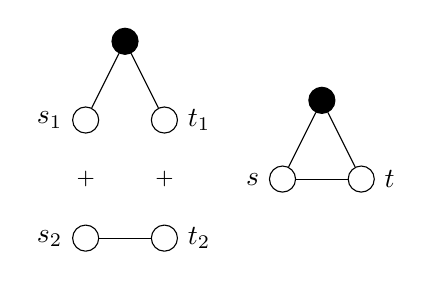
\begin{tikzpicture}
		\node[circle, draw, label=left:$s_1$] (s1) at (1,1.5) {};
		\node[circle, draw, fill=black] (v1) at (1.5,2.5) {};
		\node[circle, draw, label=right:$t_1$] (t1) at (2,1.5) {};
		
		\node[inner sep=0pt] (plus1) at (1,0.75) {\footnotesize$+$};
		\node[inner sep=0pt] (plus2) at (2,0.75) {\footnotesize$+$};
		
		\node[circle, draw, label=left:$s_2$] (s2) at (1,0) {};
		\node[circle, draw, label=right:$t_2$] (t2) at (2,0) {};
		
		\node[circle, draw, label=left:$s$] (s) at (3.5,0.75) {};
		\node[circle, draw, fill=black] (v2) at (4,1.75) {};
		\node[circle, draw, label=right:$t$] (t) at (4.5,0.75) {};
		
		\foreach \from/\to in {s1/v1,v1/t1,s2/t2,s/v2,v2/t,s/t}
		\draw[] (\from) -- (\to);
		\end{tikzpicture}
		\label{fig:spoperation:parallel}
		\subcaption{Parallel composition.}
	\end{minipage}
	\label{fig:spoperation}
	\caption{Operations on series-parallel graphs.}
\end{figure}

It follows immediately from the definition that every series-parallel graph is connected. A ``\textit{decomposition-tree}'' for a series-parallel graph displays its recursive construction according to the definition: Each tree node is a series-parallel graph and the children of each node are the subgraphs from which that graph was constructed by series or parallel composition. Figure \ref{fig:spdecomposition} shows a series-parallel graph and one of its decomposition trees. Here, the leaf $(u, v)$ denotes the series-parallel graph which consists only of the edge $(u, v)$ and the label $P(S)$ on a node stands for the series-parallel graph obtained by parallel (series) composition of its children.

\begin{figure}[H]
	\centering
	\begin{minipage}[t]{.39\linewidth}
		\centering
		\resizebox{\linewidth}{!}{%
			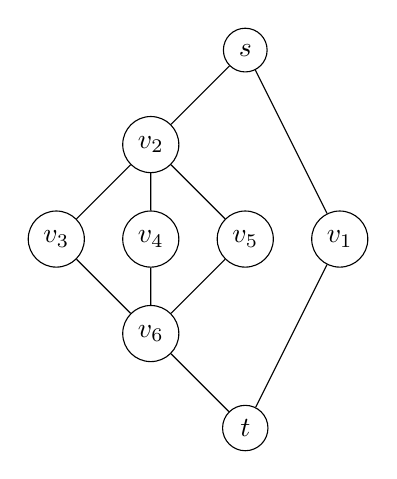
\begin{tikzpicture}
			[scale=.6,auto=middle,every node/.style={circle, draw}]
			\node (n1) at (6,8) {$s$};
			\node (n2) at (8,4)  {$v_1$};
			\node (n3) at (4,6)  {$v_2$};
			\node (n4) at (2,4) {$v_3$};
			\node (n5) at (4,4)  {$v_4$};
			\node (n6) at (6,4)  {$v_5$};
			\node (n7) at (4,2)  {$v_6$};
			\node (n8) at (6,0)  {$t$};
			
			\foreach \from/\to in {n1/n2,n2/n8,n1/n3,n3/n4,n3/n5,n3/n6,n4/n7,n5/n7,n6/n7,n7/n8}
			\draw[] (\from) -- (\to);
			\end{tikzpicture}
		}%
		\subcaption{A series-parallel graph $G$.}
	\end{minipage}
	\begin{minipage}[t]{.60\linewidth}
		\resizebox{\linewidth}{!}{%
		\begin{forest}
			[$P$,draw
			[$S$,draw
			[({$s$,}$v_2$)]
			[$S$,draw
			[$P$,draw
			[$P$,draw
			[$S$,draw
			[({$v_2$,}$v_3$)][({$v_3$,}$v_6$)]
			]
			[$S$,draw
			[({$v_2$,}$v_4$)][({$v_4$,}$v_6$)]
			]
			]
			[$S$,draw
			[({$v_2$,}$v_5$)][({$v_5$,}$v_6$)]
			]
			]
			[({$v_6$,}$t$)]
			]
			]
			[$S$,draw
			[({$s$,}$v_1$)][({$v_1$,}$t$)]
			]
			]
		\end{forest}
		}%
		\subcaption{A decomposition tree of $G$.}
	\end{minipage}
	\caption{A series-parallel graph and one of its decomposition trees.}
	\label{fig:spdecomposition}
\end{figure}

\begin{lemma}
	\label{lemma:spdecomposition}
	If $G$ is a series-parallel graph, a decomposition tree of $G$ can be constructed in time $\OO(n)$.
\end{lemma}

For the proof of Lemma \ref{lemma:spdecomposition}, we refer to \cite{VJT79}

\begin{definition}[Decomposable Graphs]
	\label{def:decompgraphs}
	Let $\Gamma$ be a class of graphs. We call the graphs in $\Gamma$ \textit{decomposable} if they are given by a set of recursive rules which satisfy the following conditions.
	\begin{itemize}
  		\item[(i)] There is a finite number of \textit{primitive} graphs in $\Gamma$, meaning only a finite number of graphs in $\Gamma$ cannot be created with the recursive rules.
  		\item[(ii)] Each graph in $\Gamma$ has an ordered (possibly empty) set of special vertices called \textit{terminals}. The number of terminals is bounded by a constant $l \in N$.
  		\item[(iii)] There are a finite number of binary composition operations $\Gamma \times \Gamma \to \Gamma$ that act only at terminals, joining terminals either by identifying two terminals or by adding an edge (called an \textit{attachment edge}) between two terminals. A
  		composition operation also determines the terminals of the resulting graph, which must be a subset of the terminals of the composing graphs. Note that the operation does not necessarily act on all terminals.
	\end{itemize}
\end{definition}

An important cautionary note: Given a graph G and a set of rules defining a class of decomposable graphs $\Gamma$, it may be a difficult problem to recognize whether or not G belongs to $\Gamma$. For the remainder of this thesis, we shall simply assume that when we are given a graph $G$ of $\Gamma$, we are also given a decomposition tree for $G$ whose size is linear in the size of $G$. In such a decomposition tree, each leaf represents a primitive graph of $\Gamma$ and each non-leaf node represents a composition operation (as well as a subgraph of $G$).

\begin{remark}
	\label{rem:spgdecomp}
	Series-parallel graphs form a class of decomposable graphs.
	\begin{itemize}
		\item The only primitive graph of the class is the graph consisting of a single edge connecting
		two different vertices.
		\item Each graph in the class has two terminals (called source and sink in Definition \ref{def:spg}).
		\item It can be seen easily that the binary operations \textit{series composition} and \textit{parallel composition}
		are of the desired kind.
	\end{itemize}
\end{remark}

Other classes of decomposable graphs are trees, outerplanar graphs, and bandwidth-$k$ graphs (\cite{BLW87}).\medskip

It can be shown that every class of decomposable graphs has a fixed upper bound on the treewidth of the graphs in the class (\cite{Wimer87}).

